\documentclass[fleqn,10pt]{physiome}
% Use option lineno for line numbers 

\articletype{Original}
%% Choose from Original, Retrospective, Review, Letter


\title{Reproducibility Study for a Computational Model of the Neurovascular Coupling Unit}

\author[1]{Sergio Dempsey}
\author[2]{Gunnar Cedersund}
\author[3,4]{Maria Engstr\"{o}m}
\author[1]{Gonzalo Maso Talou}
\author[1][soroush.safaei @auckland.ac.nz]{Soroush Safaei}
\affil[1]{Auckland Bioengineering Institute, University of Auckland, New Zealand}
\affil[2]{Department of Biomedical Engineering, Link\"{o}ping University, Link\"{o}ping, Sweden}
\affil[3]{Department of Health, Medicine and Caring Sciences, Link\"{o}ping University, Link\"{o}ping, Sweden}
\affil[4]{Center for Medical Image Science and Visualization, Link\"{o}ping University, Link\"{o}ping, Sweden}

%% The following lines can be omitted when submitting;
%% information will be added by editors
\publicationdate{21 Dec 2022}
\editor{David P. Nickerson}
\curator{Leyla Noroozbabaee}
\submitteddate{14 Sep 2022}
\accepteddate{12 Dec 2022}
\citethisas{Dempsey et al. (2022)\\Reproducibility Study for a Computational Model of the Neurovascular Coupling Unit. Physiome.}{10.36903/physiome.21714863}
\begin{document}

\maketitle

\begin{abstract}
The mechanistic model of neurovascular coupling was developed and studied by \cite{Sten2020}. This model describes and predicts the arteriolar dilation data of mice under various stimulations while anaesthetised and awake. We reconstructed the model in CellML, using a modular approach for each neuronal pathway, and successfully reproduced the original experiments (see the figures in this article and \cite{Sten2020}). With the success of the result reproduction, the CellML model can now be injected into other OpenCOR workflows to obtain a mechanistic hemodynamic response function of neurovascular coupling arteriolar dilation.
\end{abstract}

\keywords{CellML; neurovascular coupling; anaesthesia; reproducibility}

\primarypubs[https://doi.org/10.36903/physiome.21714863]{main}{Sten2020}


\section{Introduction}

Neurovascular coupling (NVC) is the cerebral pathway to modulate blood flow by manipulating local vascular tone \citep{Iadecola2017, Schaeffer2021}. This modulation is required based on the metabolic demand of the tissue, and its impairment can lead to neurodegeneration and cognitive disease \citep{Sweeney2019, Iadecola2019}. To prevent this impairment, we need a detailed understanding of the mechanisms of the NVC unit. In line with this goal, researchers have developed mechanistic mathematical models of NVC \citep{Hart2019, Sten2020} based on experiment. The mechanistic hemodynamic response functions (HRF) of the models under various stimulations are then tested against \emph{in vivo} experiments. With success, the model is then used to explore other core predictions produced increasing our knowledge of NVC and motivating further study. The model presented in \cite{Sten2020} considers GABAergic interneurons for the first time and is capable of accurately modelling arteriolar dilation data from mice under awake and anaesthetised conditions, as reported by \cite{Uhlirova2016}. 

Here, we present a CellML version of the model using the system of equations described in \citet{Sten2020} without modifications. Our CellML implementation is modular, allowing future studies to import separate pyramidal (Pyr), GABAergic Nitric Oxide (NO) and GABAergic Neuropeptide Y (NPY) control. With this model, our objective is to reproduce all steady-state variables that optimise arteriolar dilation results in \cite{Sten2020}. We omit the reproduction of confidence intervals generated by Markov Chain Monte Carlo (MCMC) simulations, since the goal is model reproducibility and reusability, not evaluation of model fidelity or sensitivity, as provided in the primary publication \citep{Sten2020}.

The proposed CellML implementation can be run in OpenCOR\footnote{\url{https://opencor.ws/}} and Python software, extending the implementation of the primary publication in MATLAB R2017b. This implementation enables more researchers to access the model.


\section{Model Description}
\subsection{Primary Publication}

The model of \cite{Sten2020} is a mechanistic model of neurovascular coupling that begins with neuronal stimulation and ends with modulation of arterial tone. The model was designed based on the iterative philosophy of systems biology, which allows quantitative experimental data to drive model development and improvement. If a proposed model can capture experimental data and is physiologically sound, then the model is accepted.

At times, an accepted model may be cumbersome due to the number of parameters and the complexity of the system. In these instances, complexity can be reduced if the model is minimised. This is the process of removing parts of the model and re-optimising to the data. This continues until the minimised model can no longer capture the data with confidence \citep{Lundengard2016}. The model presented in the primary publication is a minimised systems biology model. Interpretations of state variables can be made, but it is important to recognise that potentially multiple processes with similar responses may be lumped into one set of equations.

The model is divided into three sections, neuronal, intracellular, and vascular. In the neuronal section, each type of neuron (pyramidal, GABAergic NO, and GABAergic NPY) can receive stimulation that increases their activity. This activity can activate the other two neurons in the case of pyramidal activation or inhibit activity in the case of GABAergic interneurons. In the respective signalling pathways of neurons, activity stimulates depolarisation and a subsequent increase in calcium that activates the signalling pathway to produce vasodilatory (pyramidal and GABAergic NO pathways) or vasoconstrictive (GABAergic NPY path) factors. These final three outputs are collected and summed with respective weighting coefficients to simulate the response of the vessel. The readers are referred to the primary publication for complete details of the model \citep{Sten2020}.

The model contains a total of $13$ coupled ODEs based on mass-action, or Michaelis-Menten kinetics. The original model was implemented in MATLAB 2017b and used the third-party package AMICI\footnote{\url{https://github.com/AMICI-dev/AMICI}} to run the CVODES solver. The model was optimised using MCMC methods provided by the MEIGO\footnote{\url{https://bitbucket.org/jrbanga\_/meigo64/src/master/}} and PESTO\footnote{\url{https://github.com/ICB-DCM/PESTO}} packages. The scripts to run the original model are provided in the supplementary material of \cite{Sten2020}.


\subsection{CellML Model}

The structure of the model is built following recommended CellML best practises (see \autoref{fig:1}). This includes modularisation of the pyramidal, GABAergic NO and GABAergic NPY neuronal signalling pathways for best combined prediction or separate use. Best practises also encourage the separation of model mathematics and parameters so that one model can handle various parameter sets. For this model, the parameters simulate different neuronal dynamics. Examples that will impact neuronal dynamics include the type of stimulation, the conditions of the experiment (anaesthesia), and the genetic modulation that manifests itself as coefficient modification. We have achieved these criteria, as well as reduced the number of input parameters by including a toggle for anaesthesia versus awake conditions in our parameter files. This is a benefit compared to the five separate models required in the primary publication. This simplification also reduces the toll of scripts, allowing users to run different scenarios by only altering the set of parameters. To reproduce all results, only six parameters in the parameters file need to be modified. These six parameters define the start and stop times for stimulation, whether the unit is ``awake'' or ``anaesthetised'', and finally the stimulation scaling constants are discussed in detail in the primary publication.

The CellML model was executed with the optimised rate constants and other parameters tabulated in the supplementary material of the primary publication. These values are rounded from what was optimised in the original code; differences if any, will be discussed in the results. The CellML model is initialised using steady-state values from its own simulation run for $500$ seconds and not from the tabulated in the supplementary material. This accounts for any steady-state result errors that may have been caused by rounding. Again, the differences will be discussed in the results.

This model will be used to reproduce Figures $3$, $5$ and $6$ of the primary publication.

\begin{figure}[htbp]
    \centering
    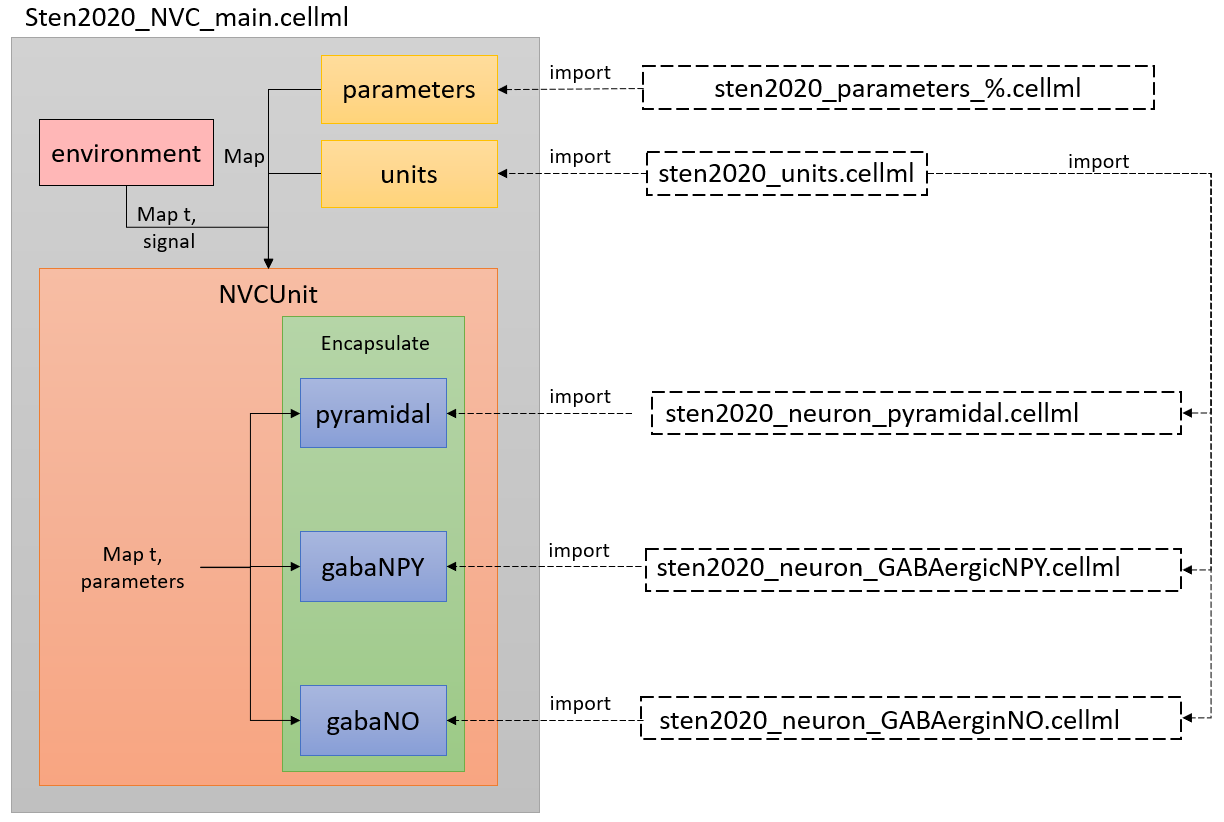
\includegraphics[scale=0.4, keepaspectratio]{Figure0.png}
    \caption{Arrangement of the model showing the CellML scripts involved. Sten2020\_NVC\_main.cellml imports components from the other scripts and constructs the model through mapping of variables between components.}
    \label{fig:1}
\end{figure}

\subsection{Clarifications and Modifications}

In Figure $3$ of the primary publication, the stimulation windows are shown in each graph, but the exact timing of neuronal stimulation is not presented in the manuscript or the supplementary materials. It is presented in the code, which we tabulate here for clarity. 

\begin{table}[htb]
    \centering
    \caption{Stimulation times to reproduce figures.}\label{table:1}
    \begin{tabular}{l l r r}
        \toprule
        Figure \# & Model Conditions & Stimulation& Stimulation\\
        (Primary) &  &  Start Time (sec) &  Length (sec) \\\bottomrule
        Figure 3  & Awake-Sensory Stim & 0 & 1\\
        & Awake-Optogenetic (GABAergic) & 0 & 0.4\\
        & Anesthesia-Sensory & 0 & 2\\
        & Anesthesia-Optogenetic (GABAergic) & 0.55 & 0.45\\
        & Anesthesia-Optogenetic (Pyramidal) & 0.9 & 0.1\\\toprule
        Figure 5/6 & Awake-Optogenetic (GABAergic) & 0 & 0.4\\
        & Anesthesia-Optogenetic (GABAergic) & 0 & 0.45\\
        \bottomrule
    \end{tabular}
\end{table}

In the reproduction of Figure $5$c, the label in $\Delta v_1=1$ is $V_\mathrm{max}$; however, the normalisation to reproduce this plot followed Equation~\ref{eqn1} below, which means $1\equiv V_\mathrm{max}-v_1^\mathrm{SteadyState}$. 

\begin{equation}
    \Delta v_1 = \frac{\frac{V_\mathrm{max}NPY(t)}{K_{M}+NPY(t)}-v_1^{\mathrm{SteadyState}}}{V_\mathrm{max}-v_1^{\mathrm{SteadyState}}}
    \label{eqn1}
\end{equation}

\begin{equation}
    v_1^\mathrm{SteadyState} = \frac{V_\mathrm{max}NPY_\mathrm{SteadyState}}{K_{M}+NPY_\mathrm{SteadyState}}
    \label{eqn2}
\end{equation}

Finally, to reproduce the plot data in Figure $6$ of the primary publication, the first row of the plots corresponding to the neuronal activity of the NPY and NO pathways is not normalised as suggested in the primary publication. We have changed the title to ``Cell Activity'', which is unitless.

\section{Model Execution}

The results were generated using the 2022-05-31 snapshot of OpenCOR \citep{Garny2015} and MATLAB R2021a to produce the plots \citep{MATLABR2021a}. The MATLAB code requires software newer than R2019b. The entire code is available at \url{https://models.physiomeproject.org/workspace/8a2}. To generate results, follow this step-wise procedure for each parameter set named in \autoref{table:2}. 

\begin{table}[htb]
\begin{center}
    \caption{Parameter set names}\label{table:2}
    \begin{tabular}{l l l}
        \toprule
        Start Text & Simulation Tag (\%\%) & End Text \\
        \bottomrule
         & Fig3A & .cellml\\
         & Fig3B & .cellml\\
         & Fig3C & .cellml\\
         sten2020\_parameters\_& Fig3D & .cellml\\
         & Fig3E & .cellml\\
         & Fig5and6\_Ana & .cellml\\
         & Fig5and6\_Awake & .cellml\\
        \bottomrule
    \end{tabular}
    \end{center}
\end{table}

\subsection{Step1: Load parameters} 
Open sten2020\_NVC\_main.cellml and on line $24$ alter the parameter name to any of the tags (\%\%) in \autoref{table:2}. All parameter filenames are in the same location as the main function and follow the naming of the figure to be reproduced from the primary publication.
\subsection{Step2: Simulation Parameters} 
The equations were solved using the CVODE solver with a maximum timestep-size equal to $0.01$. The model is already initialised in steady state. All run times are $50$ seconds with a timestep of $0.01$ seconds. 

\subsection{Step3: Export} 
When the simulation is complete, export all the data to .csv. Use the default name sten2020\_NVC\_main\_data.csv but amend the parameter case (\%\%) to the end as shown sten2020\_NVC\_main\_data\_\verb|%%|.csv. Place each csv file into an <Output CSVs> folder in the workspace. This is filled with the results by default. 

\subsection{Step4: Generate Plots} 
To reproduce the figures, run the chosen Matlab function in the folder <MatlabFiles> from within its directory. The name of the script corresponds to the figure it produces; for example, running \texttt{Figure3.m} will produce Figure $3$ in the primary publication. 

\section{Model Results}

Starting with steady-state values, only $3$ values were not identical to those published in the supplementary material of the primary publication. The steady-state values for arachidonic acid, NO, and NO$_\mathrm{vsm}$ were $6.224$, $2944.421$, and $352.127$ in the CellML model and $6.226$, $2944.636$, and $352.139$ in the primary publication; all differences are less than $0.01$\%. This led us to conclude that using the rounded numbers was safe to continue with figure reproduction.

The first figure reproduced is Figure $3$ of the primary publication shown in \autoref{fig:2}. In this figure, the results of arterial dilation are shown for $5$ different stimulus cases. The parameters used to produce this graph come from the best-fit parameters in the primary publication. All subplots agree with the primary publication. 

\begin{figure}[htbp]
    \centering
    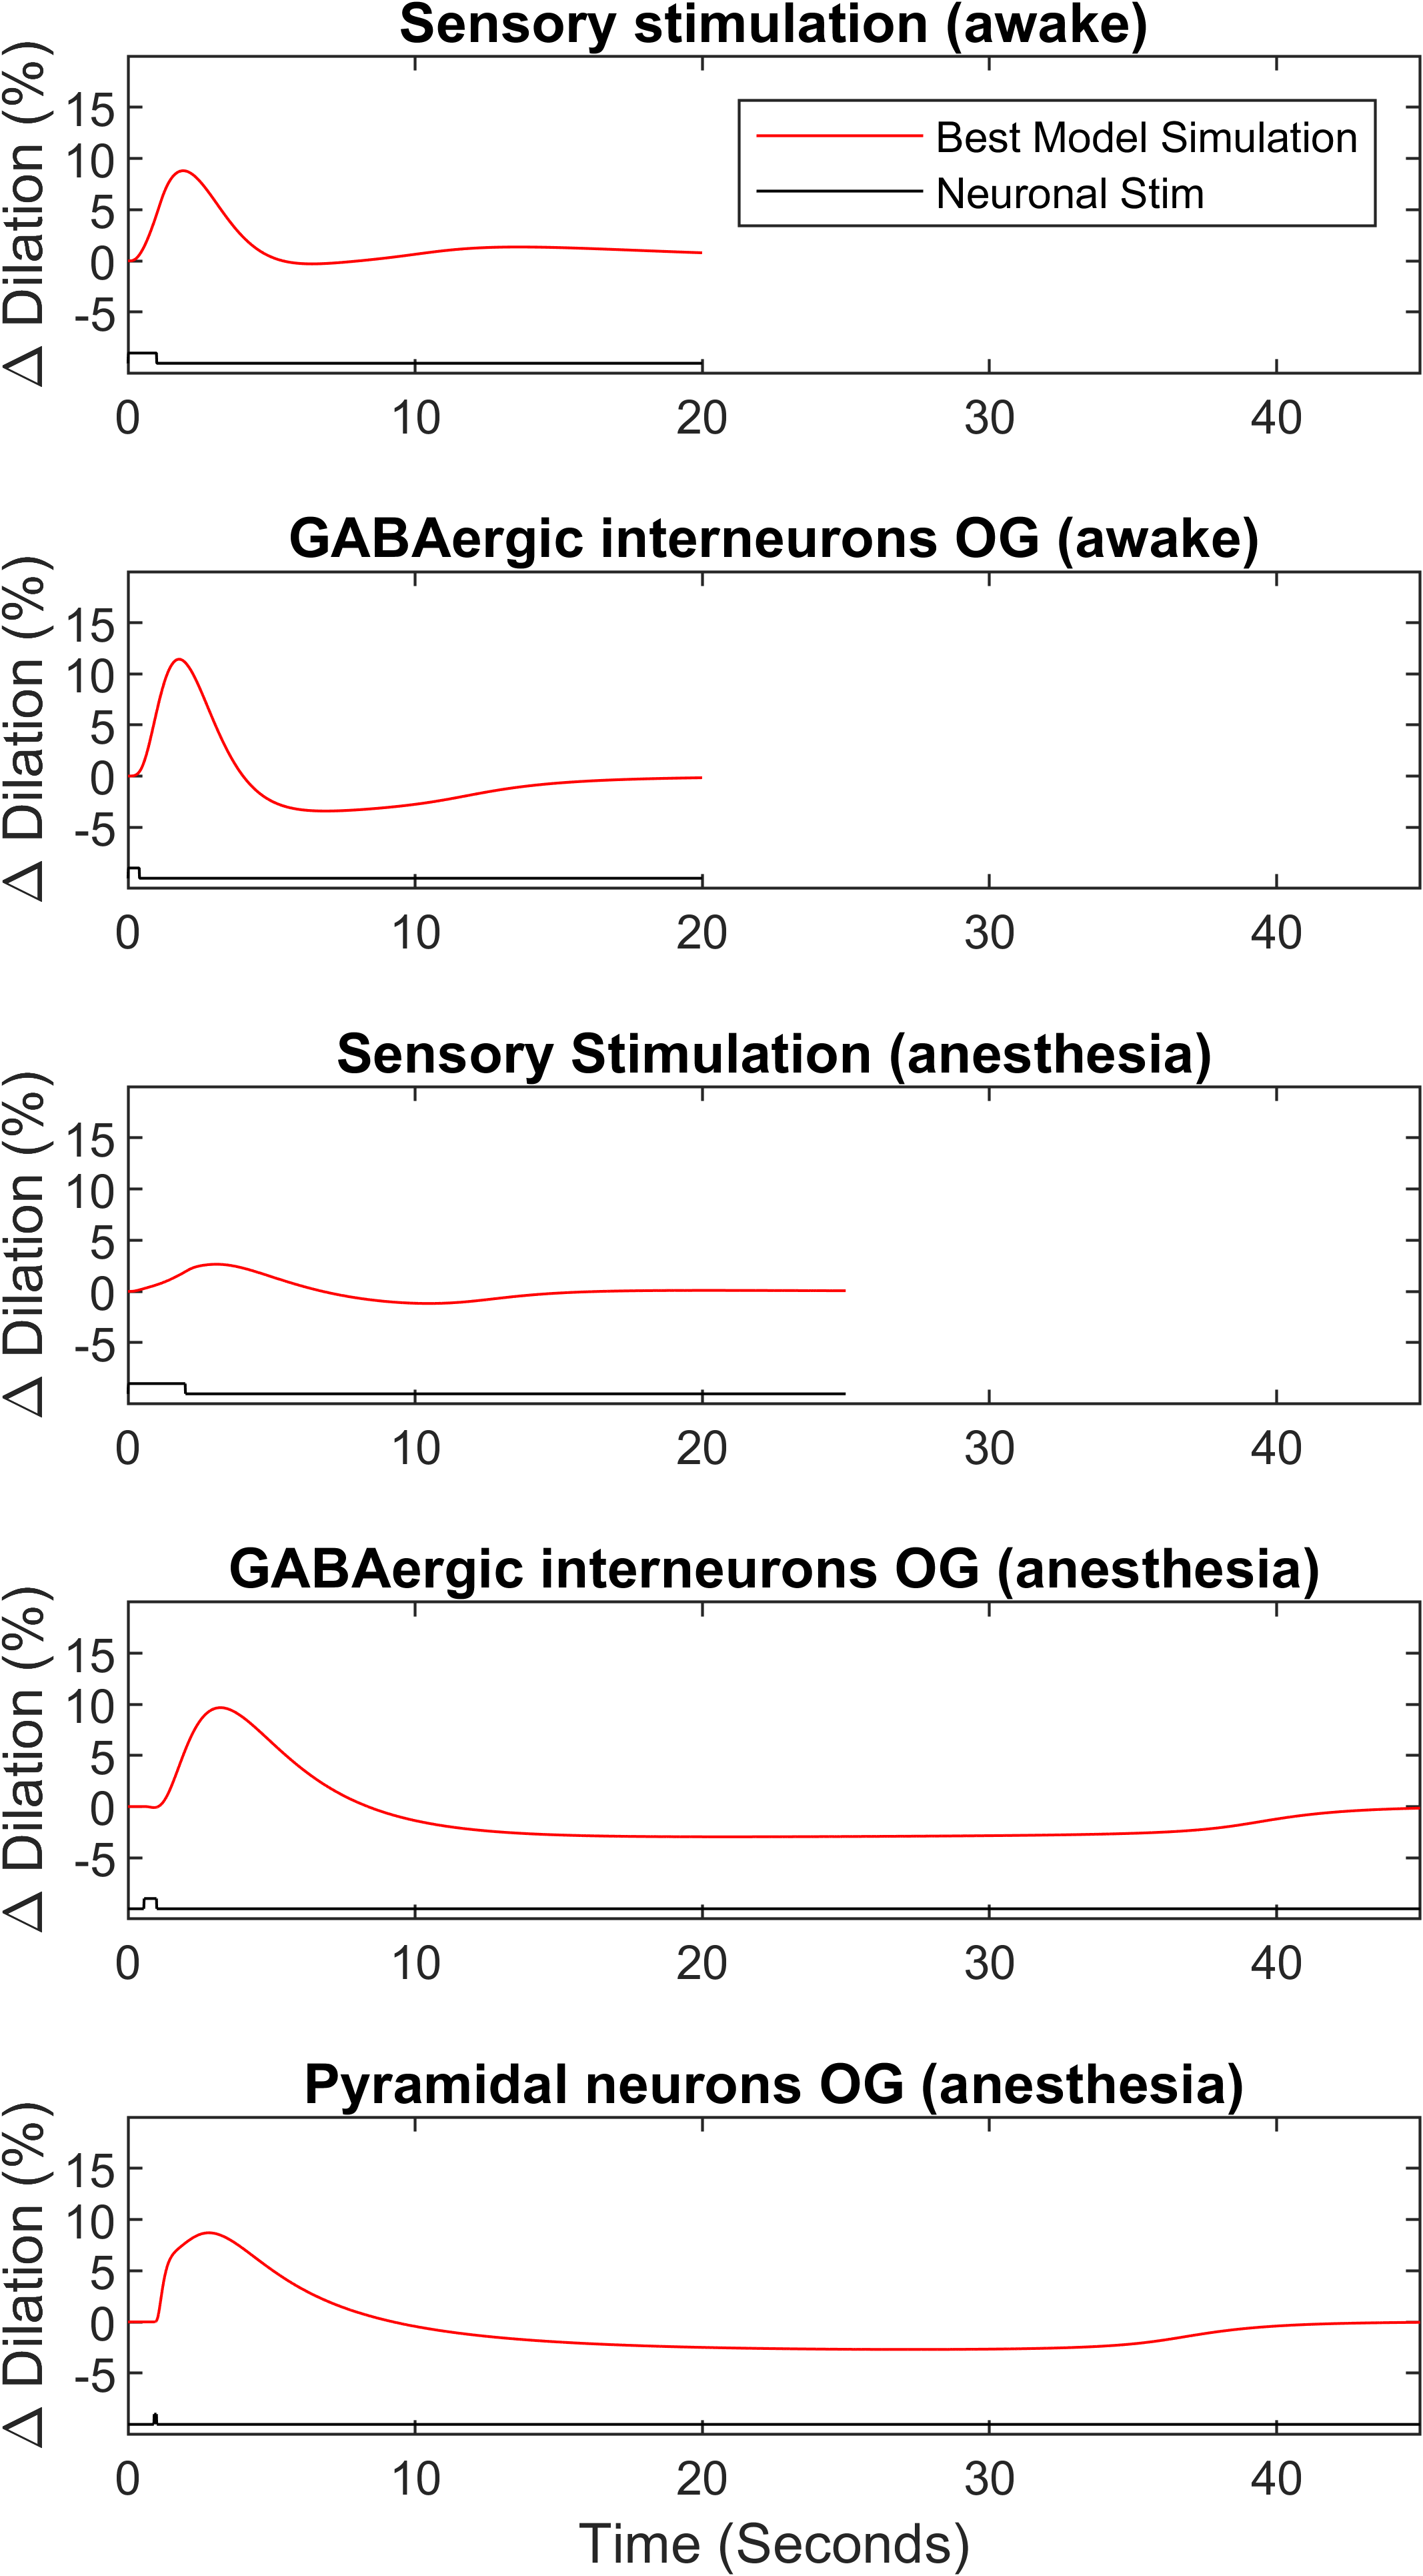
\includegraphics[scale=0.7,keepaspectratio]{Figure3.png}
    \caption{Best estimated model simulation of arteriolar dilation to sensory or optogenetic stimulation in awake and anesthetised mice. This figure matches the subfigures B-D-F-H-J of Figure $3$ in the primary publication and can be reproduced using \texttt{Figure3.m} file.}
    \label{fig:2}
\end{figure}

The second figure reproduced is Figure $5$ of the primary publication shown in \autoref{fig:3}. This figure emphasises the impact of using Michaelis-Menten kinetics for the production of NPY in vascular smooth muscle (vsm). All subplots agree with the primary publication. 

\begin{figure}[htbp]
    \centering
    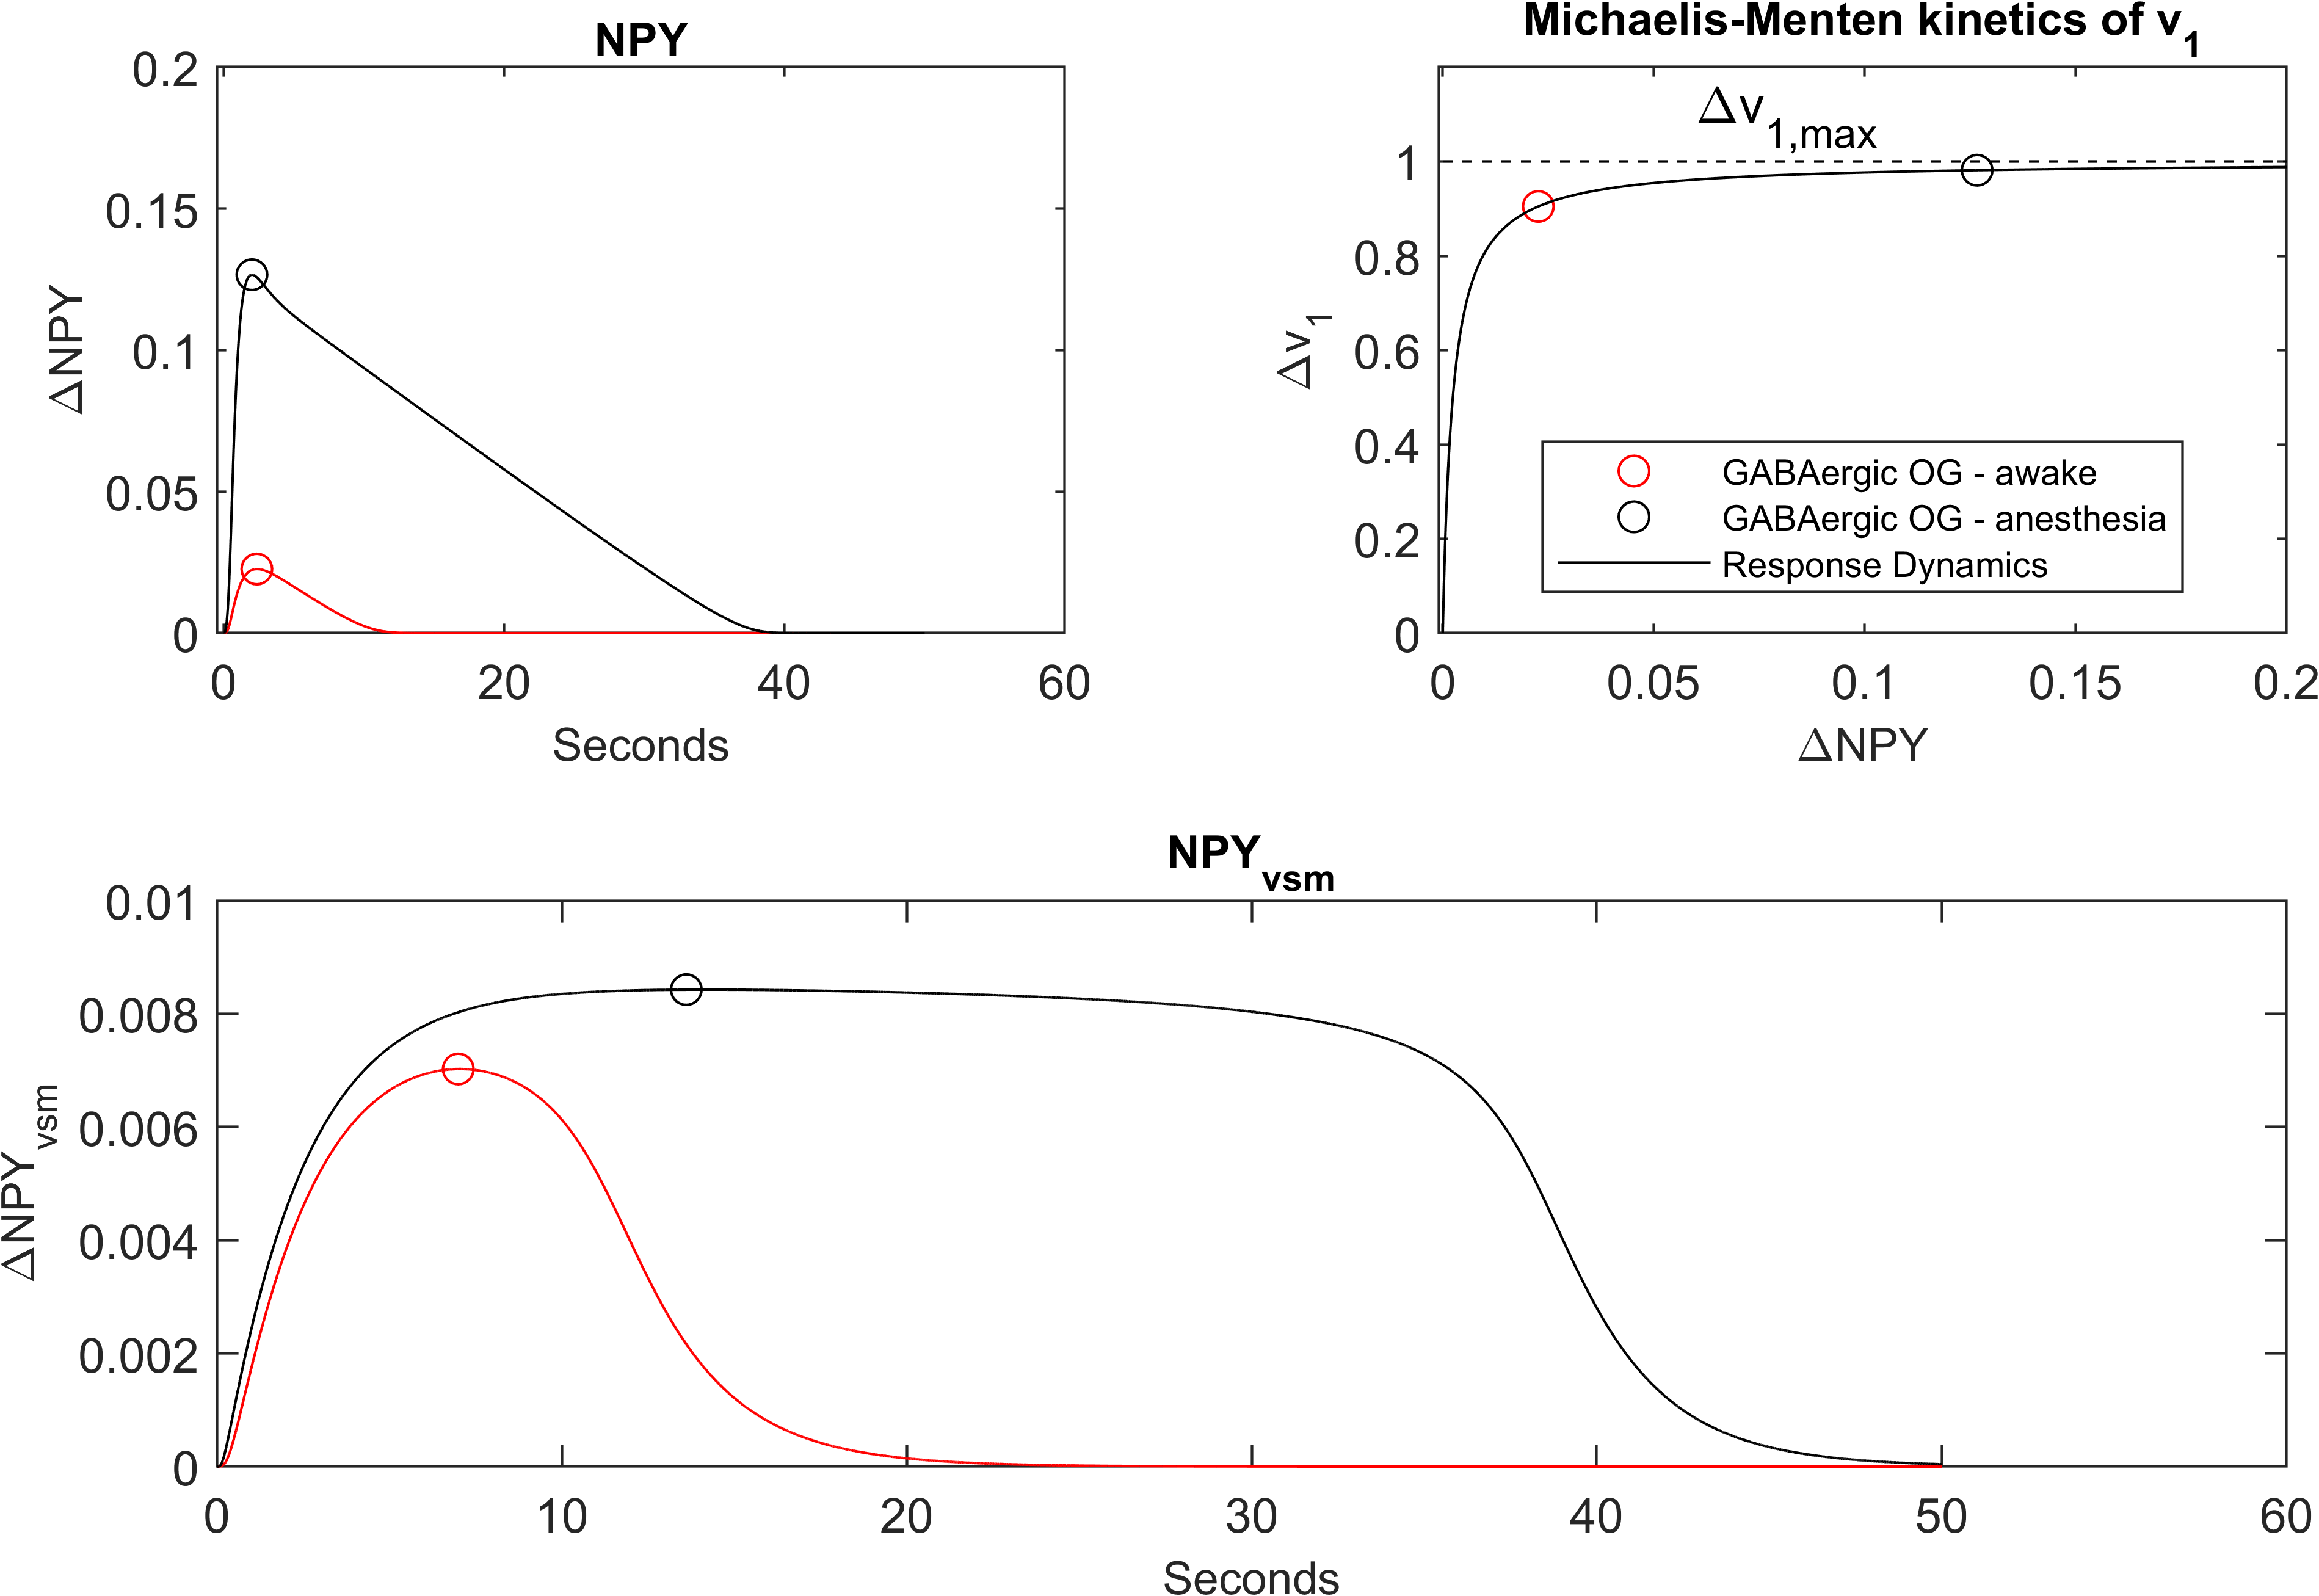
\includegraphics[scale=0.8, keepaspectratio]{Figure5.png}
    \caption{NPY response from optogenetic stimulation of GABAergic interneurons in awake and anesthetised mice. (top left) Change in NPY from baseline steady state for awake and anesthetised optogenetic GABAergic stimulation. (top right) Change in rate of NPY$_\mathrm{vsm}$ production as a function of NPY produced from baseline showing minor changes in rate for large increases in production in anesthetised vs awake conditions. (bottom) Change in NPY$_\mathrm{vsm}$ over time for anesthetised and awake stimulation. This figure matches the subfigures B-C-D of Figure $5$ in the primary publication and can be reproduced using \texttt{Figure5.m} file.}
    \label{fig:3}
\end{figure}

The last reproduced figure is Figure $6$ of the primary publication shown in \autoref{fig:4}. This figure shows the difference in all state variables of the GABAergic NO and NPY pathways for awake and anaesthetised conditions, highlighting that the prolonged undershoot of the anaesthetic response is due to the Michalis-Menten kinetics of NPY$_\mathrm{vsm}$. It also shows the impact of NO and its initial vasodilatory effect. For a complete interpretation and all acronyms, see the primary publication. All sub-plots agree with the primary publication. 

\begin{figure}[hbtp]
    \centering
    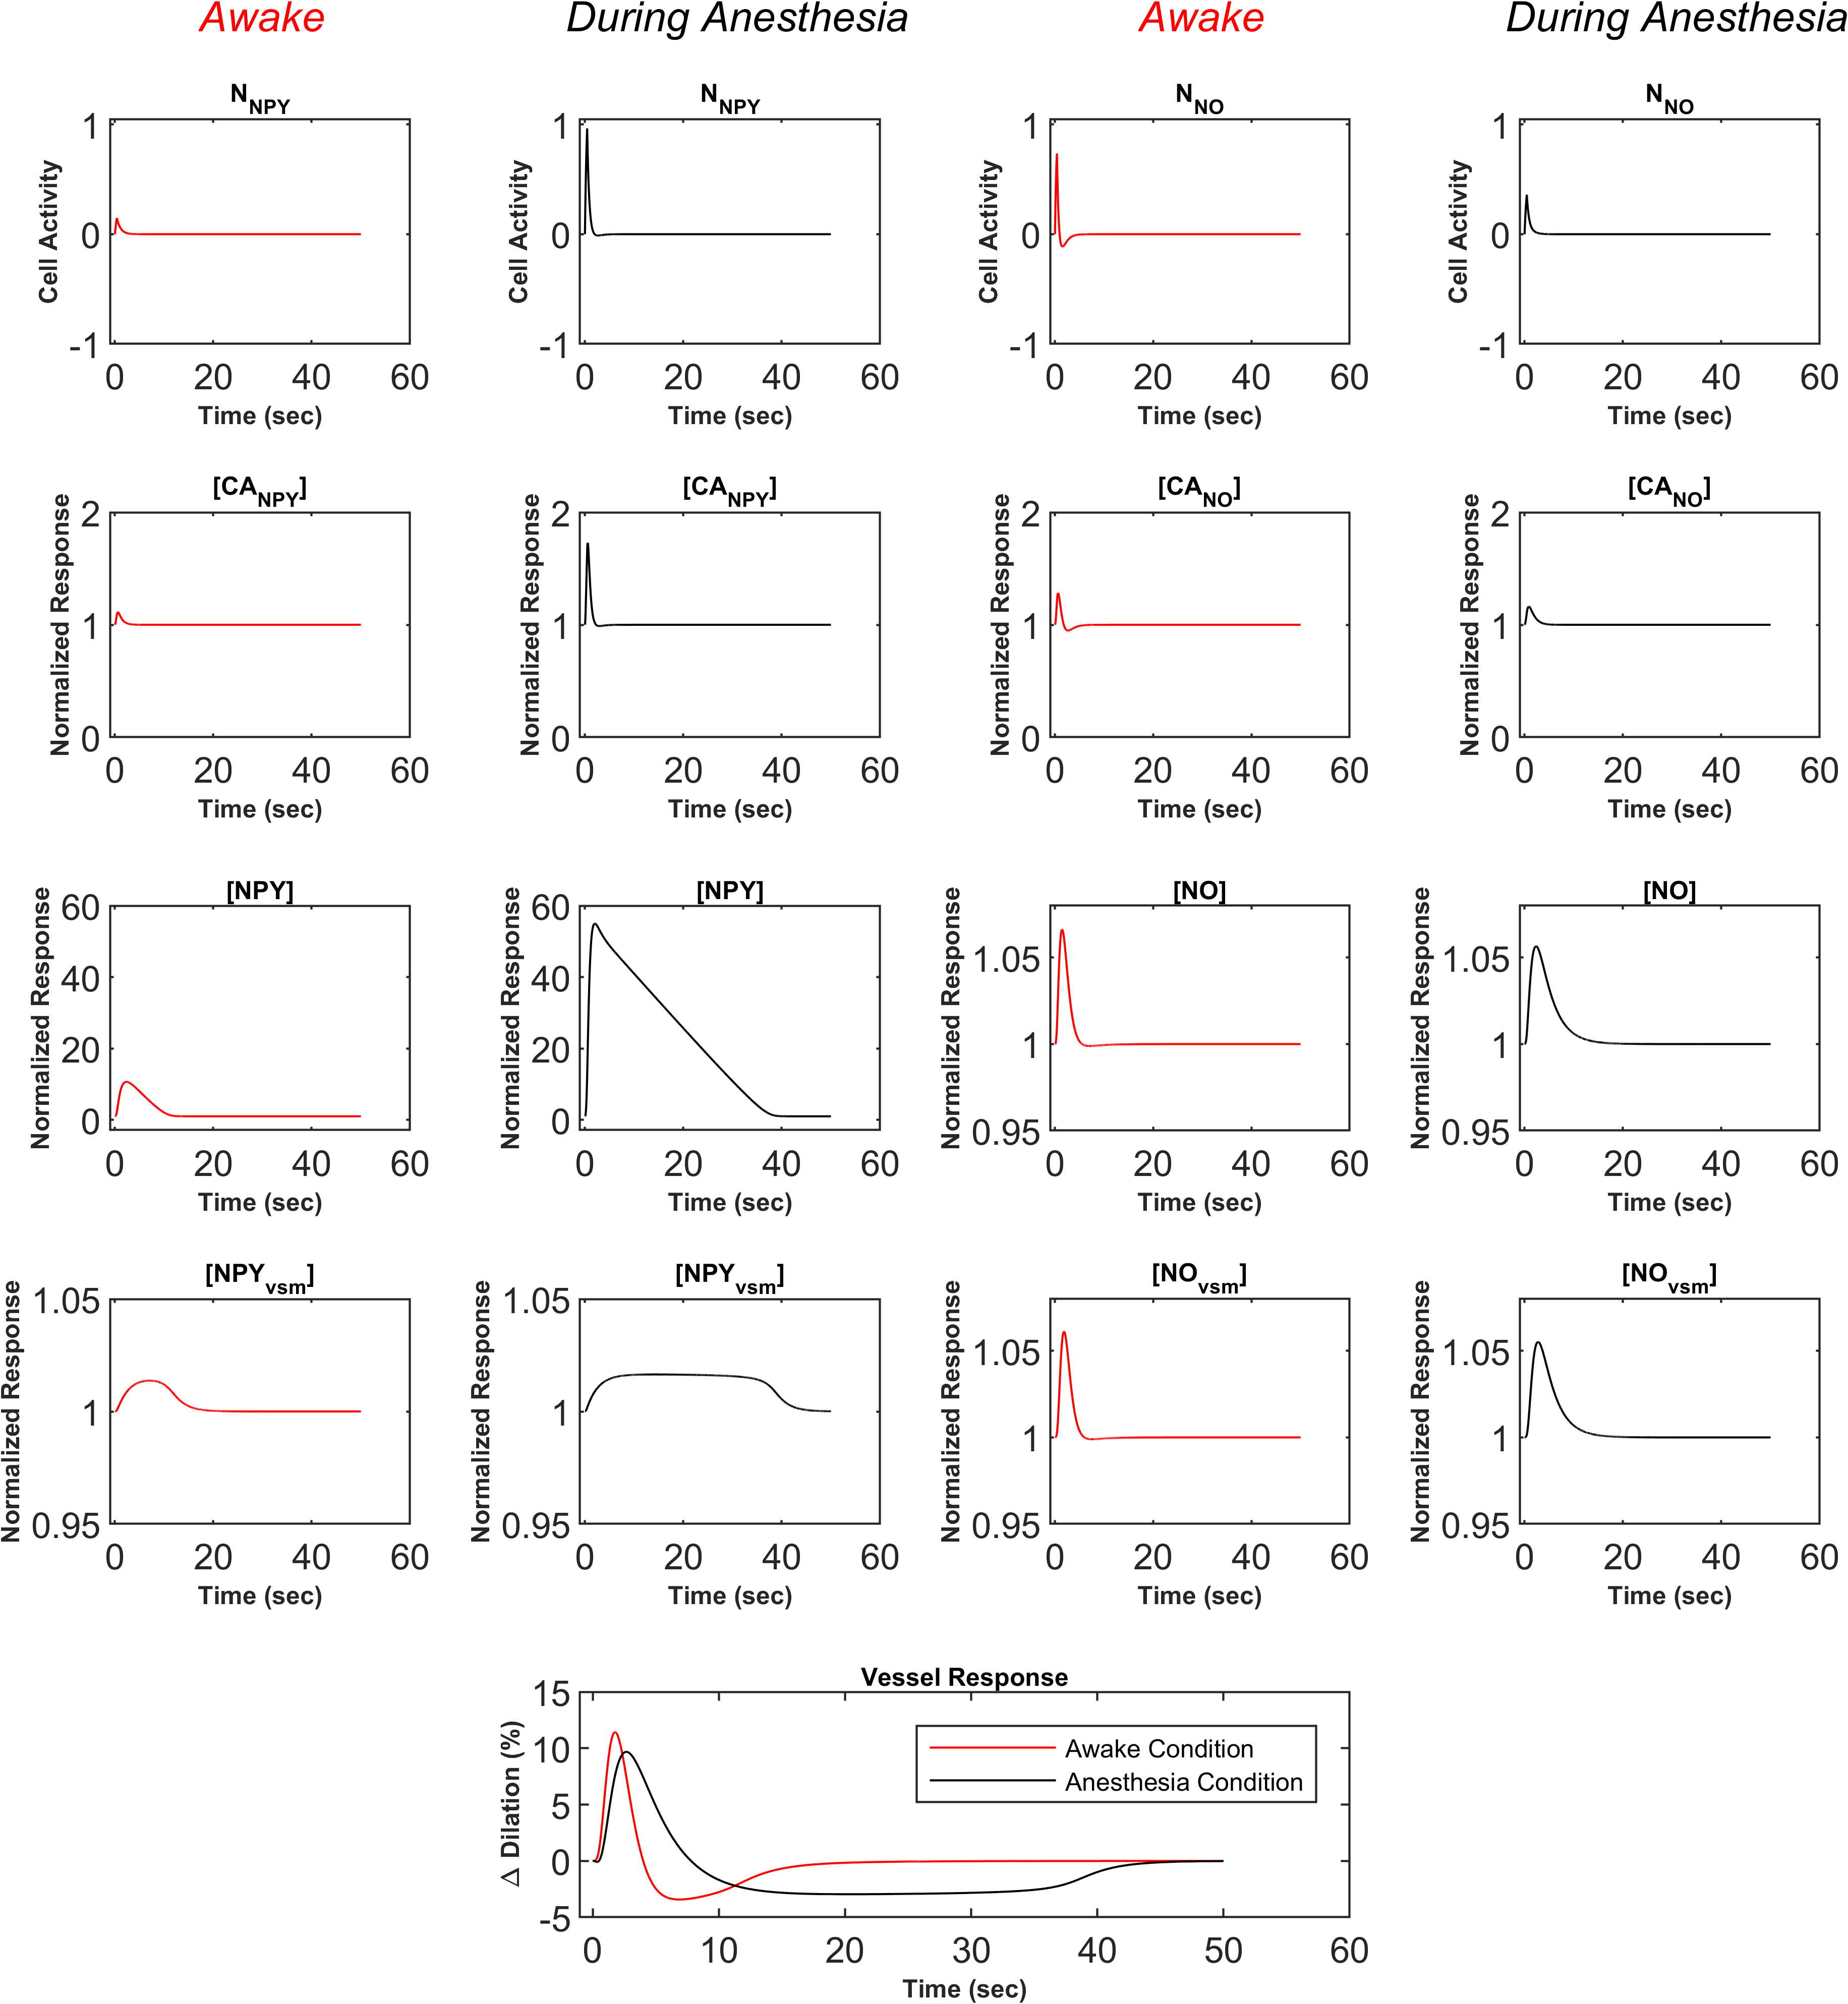
\includegraphics[scale=0.9, keepaspectratio]{Figure6.png}
    \caption{Complete presentation of the NO and NPY state variables for optogenetic stimulation of GABAergic interneurons in awake (red) and anesthetised (black) mice. This figure matches Figure $6$ in the primary publication and can be reproduced using \texttt{Figure6.m} file.}
    \label{fig:4}
\end{figure}

\section{Discussion}

In this paper, we present the CellML version of an NVC model originally developed by \cite{Sten2020} for NVC. Our implementation is modular and can be tuned to many coupling scenarios without the main code modification. Figures illustrating the model predictions from the primary publication were produced without error, and only minor clarifications are made to the titles in the primary publication's figures.


\bibliography{main}

\end{document}